\begin{enumerate}[leftmargin=*,label=\textbf{\thesection.\arabic*}]
    \item Find undirected contacts stored in the \textit{app contact} relationship.
    \begin{figure}[h]
        \centering
        
\includegraphics[width=\textwidth]{images/find_indirected_app_contacts.png}
    \end{figure} 
    \item Find the mean age of the infected\footnote{We refer to infected people as the positive-tested in the last ten days.} people in the last ten days.
    \begin{figure}[h]
        \centering
        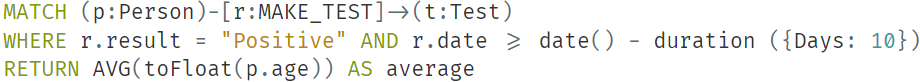
\includegraphics[width=\textwidth]{images/avg_positive_age.png}
    \end{figure} 
    \item Find people that live with someone who has been tested positive in the last ten days.
    \begin{figure}[h]
        \centering
        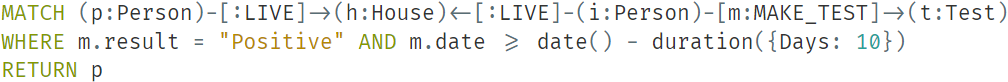
\includegraphics[width=\textwidth]{images/mates_of_positives.png}
    \end{figure} 
\item Find the houses where resides someone tested positive in the last ten days.
    \begin{figure}[!htb]
        \centering
        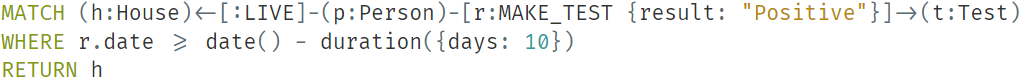
\includegraphics[width=\textwidth]{images/homes_with_positive.png}
    \end{figure}
\newpage
    \item Find the number of test performed in the last month.
    \begin{figure}[h]
        \centering
        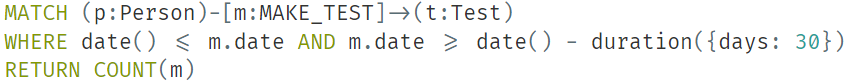
\includegraphics[width=\textwidth]{images/tests_last_30_days.png}
    \end{figure} 
    \item Find the number of infected people in a given month.
    \begin{figure}[h]
    \centering
        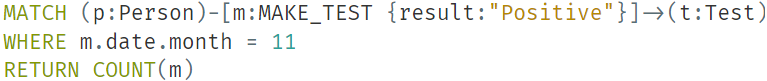
\includegraphics[width=\textwidth]{images/positives_given_month.png}
    \end{figure} 
    \item Find the number of vaccinations performed in a given month.
    \begin{figure}[h]
        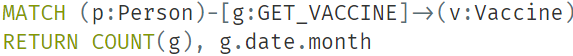
\includegraphics[scale = 0.7]{images/vaccinated_per_month.png}
    \end{figure}     
    \item Find the number of people with a single vaccine dose.
    \begin{figure}[!htb]
        \centering
        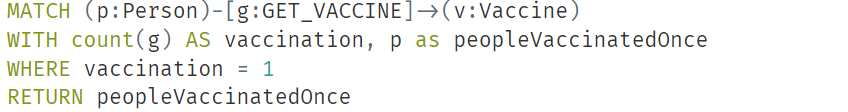
\includegraphics[scale = 0.7]{images/vaccinated_once.png}
    \end{figure} 
    \item Find the number of people vaccinated by CAP.
    \begin{figure}[!htb]
        \centering
        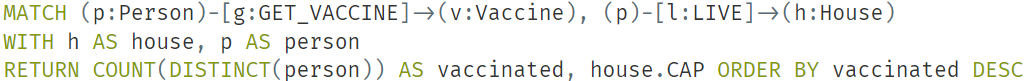
\includegraphics[width=\textwidth]{images/vaccinated_per_cap.png}
    \end{figure} 
    \item Find the first five places according to the rate of positive people in the last month.
    \begin{figure}[!htb]
        \centering
        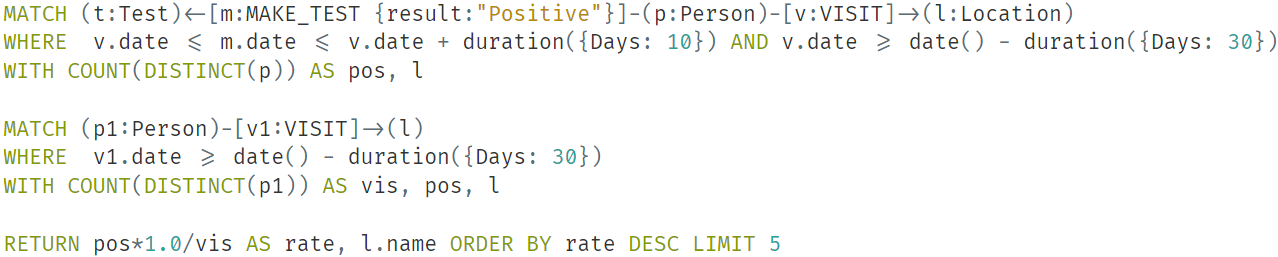
\includegraphics[width=\textwidth]{images/top_5_locations.png}
    \end{figure}
\newpage
    \item Find the people exposed to the virus who have not been tested yet.\footnote{They haven't made a swab from the date of the last covid exposure until now.}
    \begin{figure}[!htb]
        \centering
        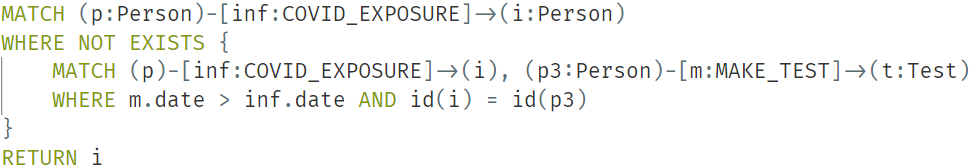
\includegraphics[width=\textwidth]{images/exposed_not_tested.png}
    \end{figure} 
    \item Find the percentage of infected people that got at least one dose of vaccine.
    \begin{figure}[h]  
        \centering
        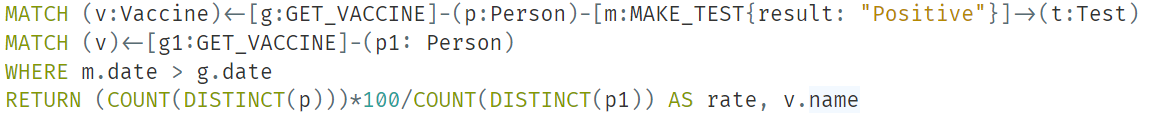
\includegraphics[width=\textwidth]{images/positive_after_vaccine.png}
    \end{figure}
    \item Find the number of people positive after being exposed to the virus.
    \begin{figure}[h]  
        \centering
        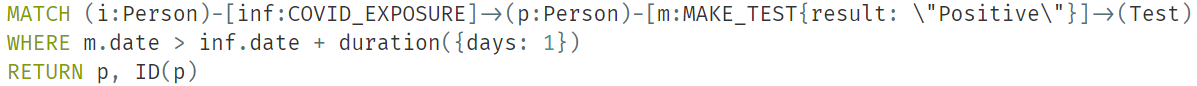
\includegraphics[width=\textwidth]{images/positive_after_exposure.png}
    \end{figure}
    \item Find not vaccinated people.
    \begin{figure}[!h]  
        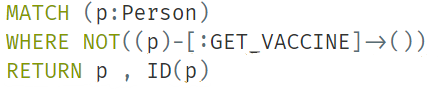
\includegraphics[scale = 0.65]{images/not_vaccinated.png}
    \end{figure}
    \item Find the number of contact detected by a tracking application for ten people.
    \begin{figure}[!h]  
        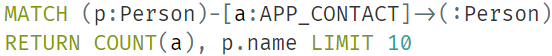
\includegraphics[scale = 0.65]{images/appcontacts_for_10_people.png}
    \end{figure}
    \item Find the worst case of covid exposures tree caused by a positive person.
    \begin{figure}[!h]  
        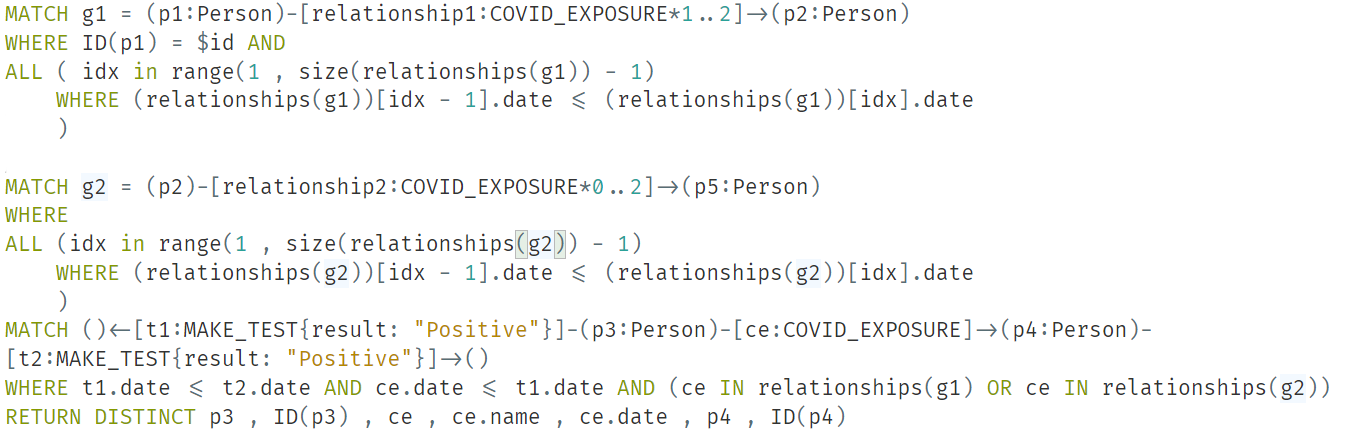
\includegraphics[width=\textwidth]{images/worst_tree_of_exposures.png}
    \end{figure}
\end{enumerate}